\documentclass[12pt]{article}

\usepackage[utf8]{inputenc}
\usepackage[T1]{fontenc}
\usepackage[top=2cm, bottom=3cm, left=3cm, right=3cm]{geometry}
\usepackage{url}
\usepackage{graphicx}
\title{Chabi Protocole}
\author{
  Cecilia BITOUT, Krimo HAMADI, Pin WANG, \\
  Jérôme SKODA et Joaquim LEFRANC
}

\date{2017}

\begin{document}
\fontfamily{cmr}
\maketitle
\section{Architecture}

\textbf{ATTENTION : Dans tout ce qui suit, le mot ``client'' est utilisé au sens de
client TCP, la distinction entre annonceur et utilisateur n'est pas faite.
La distinction peut si besoin être faite avec ``Client annonceur''}
\newline


\section{Adresse IP et port}

\begin{itemize}
  \item~Le port TCP utilisé est le 1027
  \item~IP UDP Multicast: 224.4.4.4
  \item~Port UDP Multicast : 4444
\end{itemize}






Architecture client/serveur

Serveur:
Stoque les annonces reçues
Envoie les annonces non obsoletes des clients connectés au serveur






Client:
Choisi une des petites annonces proposées par le serveur
(Entre en communication directe avec l'annonceur)

Connexion avec le serveur avec [BonjourChabi]


Conexion

Client qui se connect au serveur

Le serveur ajoute le client dans une liste et lui attribu un ID.

Deconnexion

Le client envoie un [QUIT] ou est déconnecté suite à un timeout.

Toute les annonce du client devienne obsoletes (et donc supprimé)


Poster un annonce

Un client peux créer une annonce en envoyant un

[ANN id\_client titre prix type description]

le serveur répond

[CHABI id\_annonce]


Messagerie

Pour envoyer un message vers un client annonceur, il faut envoyer un
[MES id\_client message]

 au serveur. Le serveur s'occupera de transmetre le message à l'annonceur.

Detruire une annonce

Le client envoie un [DESTROY id\_annonce]
Si l'id client et l'id\_annonce correspondent alors l'annonce est supprimé.






\section{Diagramme de connexion au serveur}

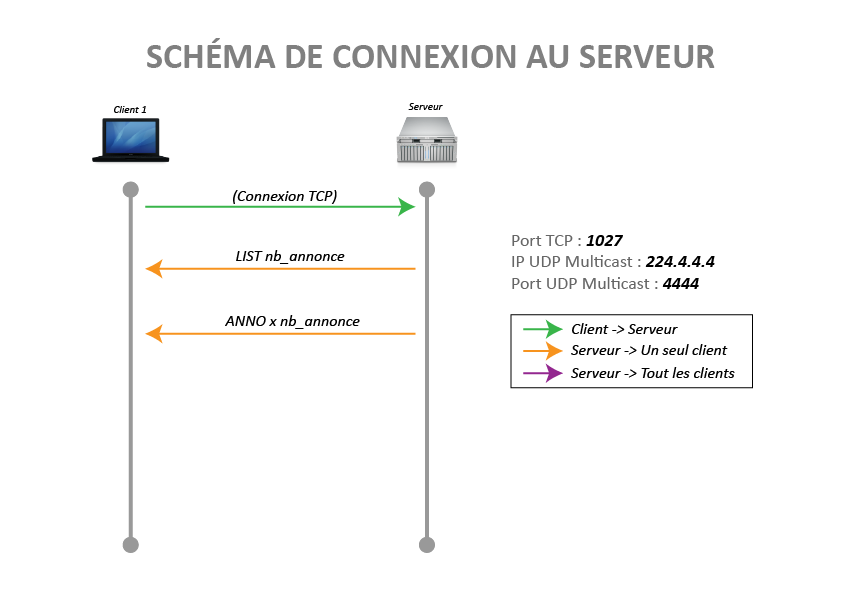
\includegraphics[width=\textwidth]{rendu1/Protocole_Connection.png}

\section{Diagramme des opérations}

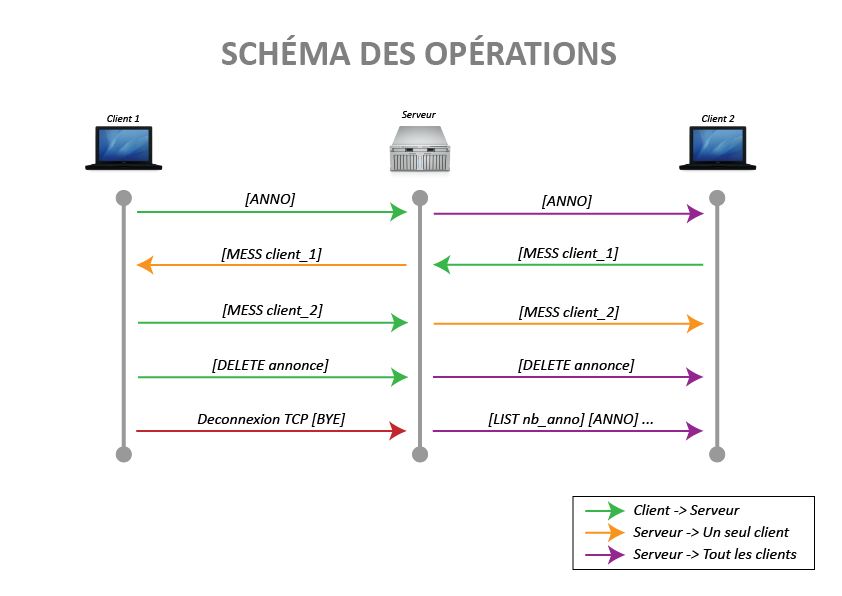
\includegraphics[width=\textwidth]{rendu1/Protocole_Operations.png}


\section{Format des messages}

Les messages sont tous encadrée de braquet "[" et "]".

Le premier mot à l'interrieur des braquets est un préfix indiquant le type de message, ils sont conventionnelement ecrit en majuscule.

Certain message contienne des arguments. Chacun de ces arguments sont séparé par des espaces, s'ils contiennent des espace il doit être
entouré de double quôte. (Fonctionnement similaire aux argv)

\begin{itemize}
  \item~[WELC] Message de bienvenue lors de la connexion d'un client via TCP
  \item~[NEWC] Requête nouveau client
  \item~[ACKC] Aquitement de nouveau client
  \item~[BYE]  Déconnexion d'un client
  \item~[ANNO~id\_annonce~id\_src~annonce\_titre~annonce\_contenu~annonce\_prix]
  \begin{itemize}
    \item id\_annonce : <int>  id unique de l'annonce (à 0 s'il s'agit d'une création d'annonce)
    \item id\_src: <int> id unique de l'annonceur (à 0 s'il s'agit d'une création d'annonce)
    \item annonce\_titre : <string> titre
    \item annonce\_contenu : <string> contenu
    \item annonce\_prix : <double> prix
  \end{itemize}
  \item~[LIST][ANNO][ANNO]...[ANNO][ENDLIST]
  \item~[MESS id\_src id\_dst client\_message]
\end{itemize}

\end{document}
